\section{Arquitectura del M\'odulo Digital}
\begin{figure}[!htb].
    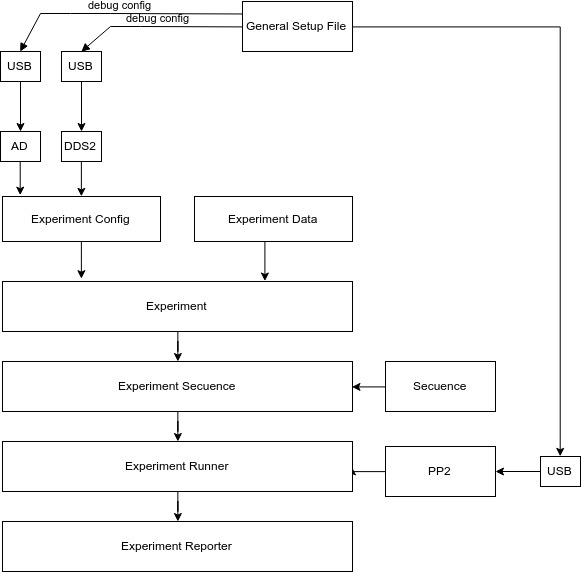
\includegraphics[width=\linewidth]{../figures/d19.jpg}
    \caption{Arquitectura M\'odulo Digital}
    \label{fig:d19}
\end{figure}

Entre las clases principales dentro del \textit{M\'odulo Digital} se destaca \textit{Experiment Reporter}
que es el \'ultimo eslab\'on de una cadena de especializaciones la cual implementa el m\'etodo "Next" de las clases
de Python, en consecuencia a la naturaleza iterable de los experimentos. 
Una instancia de esta clase tiene un comportamiento diferenciado seg\'un se trate de un experimento simulado \'o no simulado, dictaminado por el estado de la propiedad \textit{simulation-mode} definida en \textit{General Setup File}.

\newpage